\documentclass[11pt]{article}
\usepackage[margin=1in]{geometry}
\usepackage{graphicx}
\usepackage{amsmath}
\usepackage{float}
\usepackage[hidelinks]{hyperref}
\usepackage{enumitem}
\usepackage{listings}
\usepackage{xcolor}

\lstdefinestyle{matlabstyle}{
    language=Matlab,
    basicstyle=\ttfamily\small,
    breaklines=true,
    columns=fullflexible,
    frame=single,
    keepspaces=true,
    showstringspaces=false,
    keywordstyle=\color{blue},
    commentstyle=\color{teal!70!black},
    stringstyle=\color{orange!60!black}
}

\lstset{style=matlabstyle}

\begin{document}

\begin{center}
{\LARGE ME 656: Autonomous Navigation for Mobile Robots}\\[0.5em]
{\Large Simulation Lab 1 Report}\\[1em]
\begin{tabular}{ll}
Course: & ME 656 - Autonomous Navigation for Mobile Robots \\
Semester: & Spring 2026 \\
Assignment: & SimLab 1 \\
Student: & Matthew Lepis \\
\end{tabular}
\end{center}

\vspace{1em}

\section{Overview}
This report summarizes the five requested deliverables for SimLab 1. All simulations
were run with the assignment parameters: a 10 m hallway, a sensing range of 0.5 m,
landmarks at 2 m, 5 m, and 8 m, a time step of 0.1 s, and a robot speed of 0.1 m/s. For
every simulation, the estimator was evaluated over $N=1000$ Monte Carlo trials and
compared against the known ground truth trajectory.

The least squares approach solves for the full trajectory in batch form, while the
Kalman filter approach estimates the state incrementally over time. In all cases, the
reported error metric is the mean absolute robot position error as a function of time.

\section{Deliverable 1: Batch Least Squares with Odometry Only}
For the first simulation, the batch least squares problem was built using only the initial pose
constraint and the odometry displacement equations between sequential robot position
states. In this simulation variant, no landmark observations are included, therefore the estimate
is driven solely by noisy odometry measurements.

\begin{figure}[H]
\centering
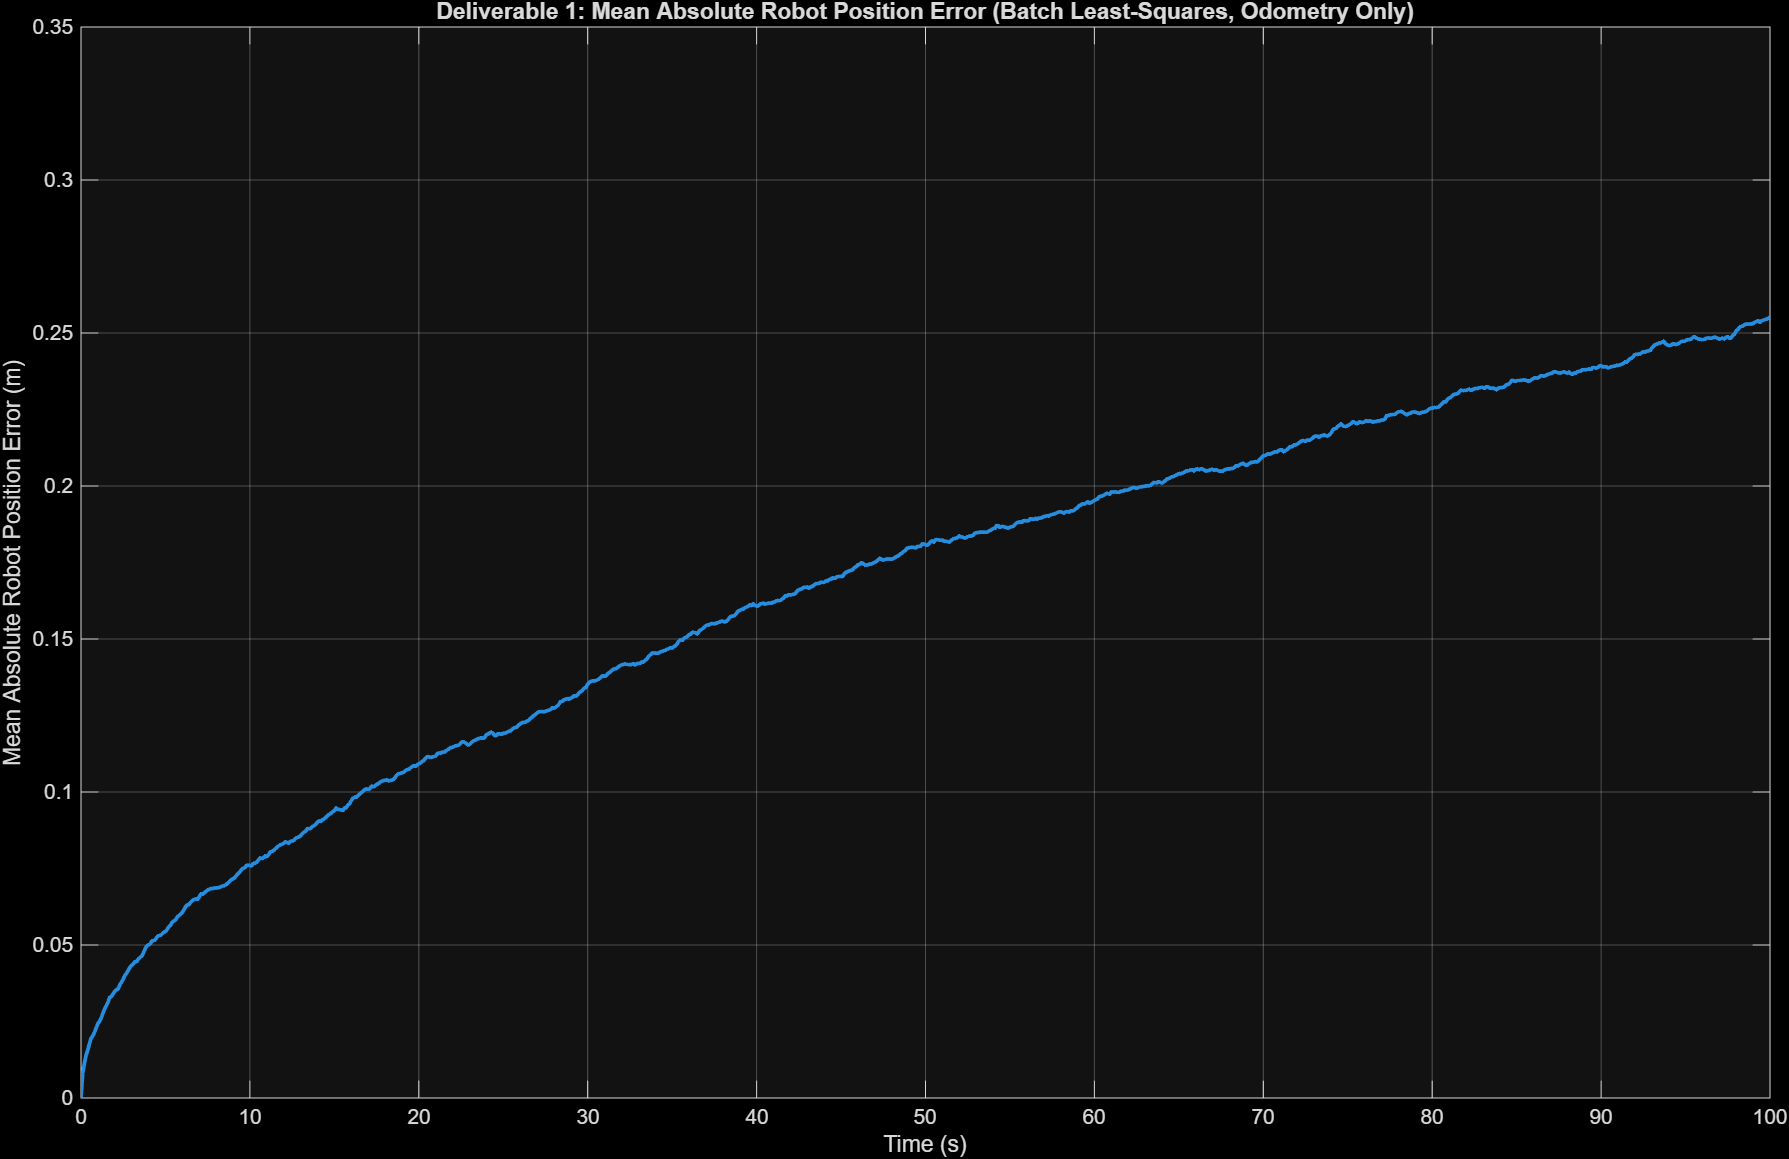
\includegraphics[width=0.9\textwidth]{Deliverable1.png}
\caption{Deliverable 1: Mean absolute robot position error for batch least squares with odometry only.}
\end{figure}

The mean absolute error grows with time because the robot never receives external
positional correction. Each noisy odometry measurement contributes a small amount of
drift, and the accumulated error becomes larger as the robot moves farther down the
hallway.

\section{Deliverable 2: Batch Least Squares with Odometry and Landmark Sensing}
In the second simulation, the batch least squares formulation was extended to include signed
landmark range measurements of the form $l_j - x_k$ (landmark [j] position minus robot position
state [k]). This keeps the measurement model linear while allowing the batch solve to 
estimate both the robot trajectory and the three landmark positions.

\begin{figure}[H]
\centering
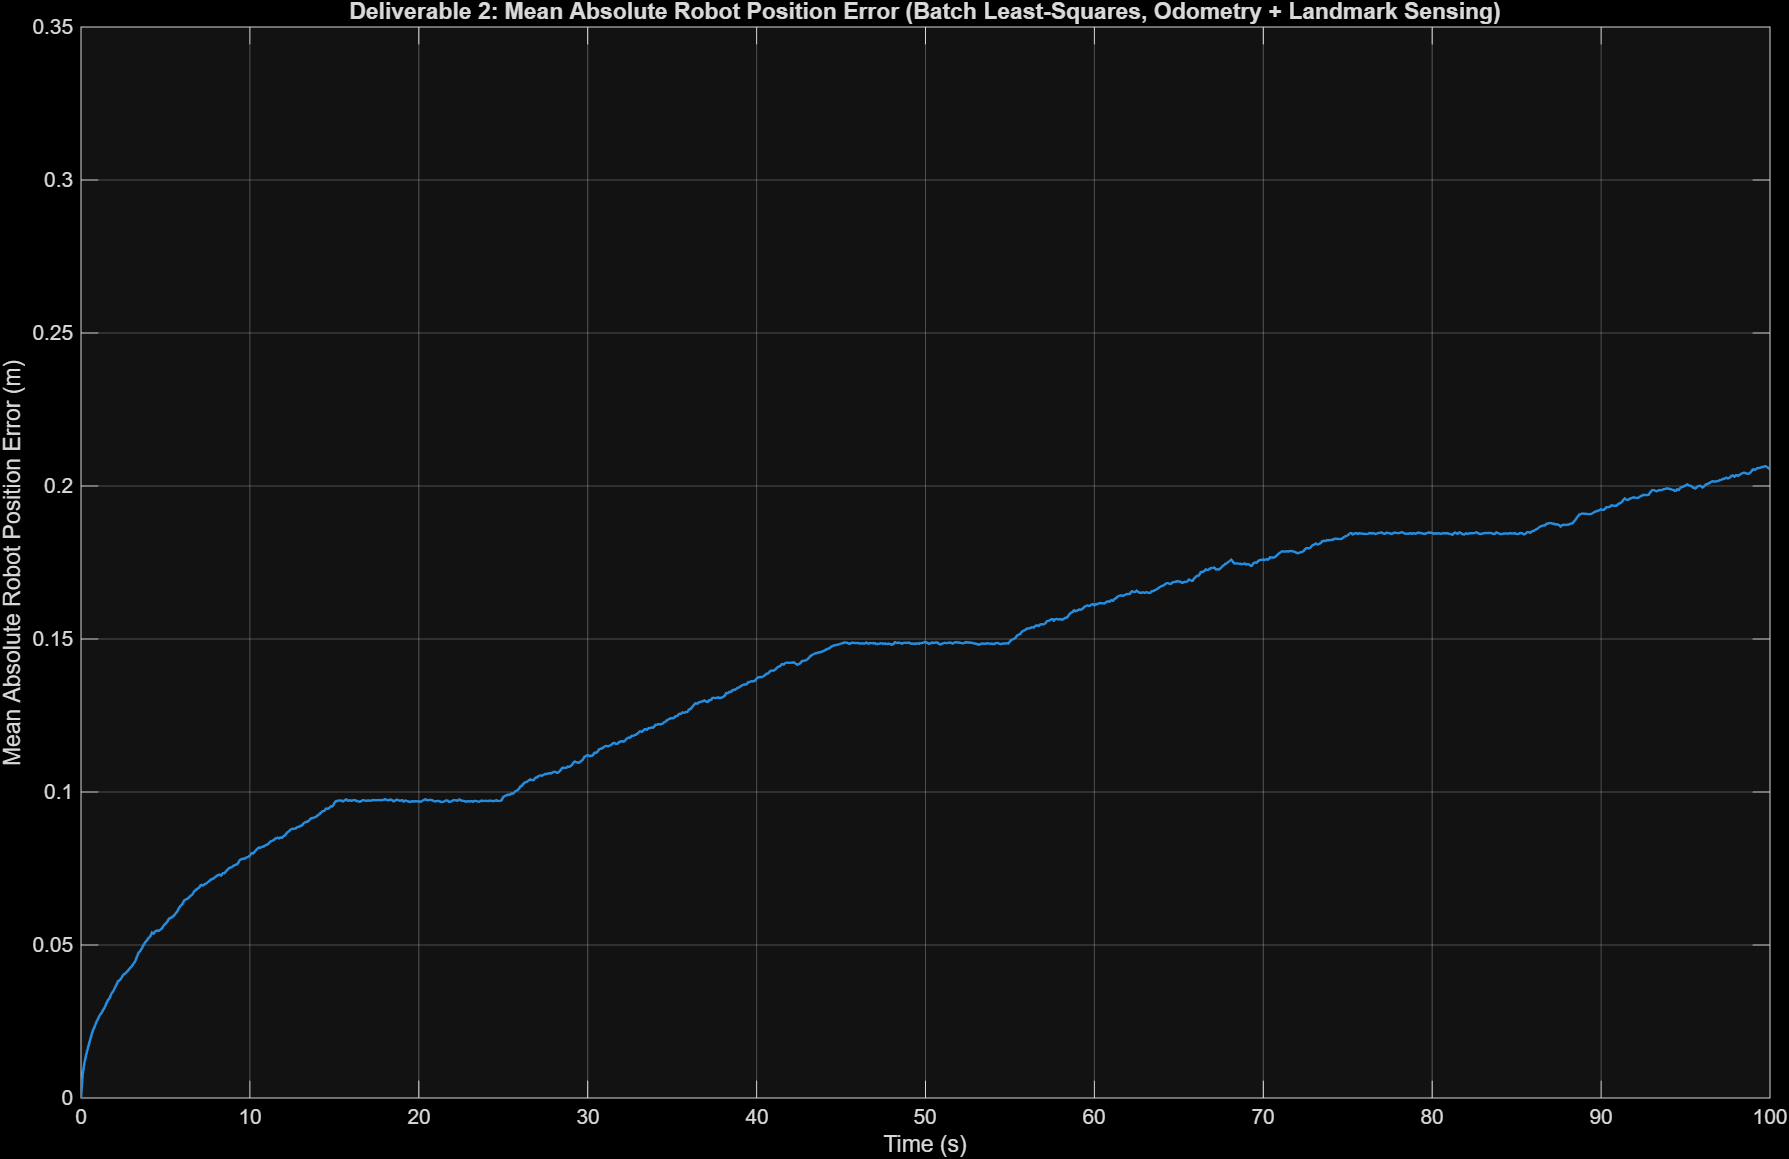
\includegraphics[width=0.9\textwidth]{Deliverable2.png}
\caption{Deliverable 2: Mean absolute robot position error for batch least squares with odometry and landmark sensing.}
\end{figure}

The introduction of the robot's observation of landmarks reduces the growth of mean error.
When landmarks are observed, the batch system gains additional constraints that tie the robot's 
pose states to fixed features in the hallway. This limits the amount of odometry drift that can
accumulate and keeps the mean absolute error lower than in the odometry-only case. Between the odometry-only
case and odometry + landmark case, this case had a ~19\% decrease in peak mean position error.

\section{Deliverable 3: Kalman Filter with Odometry Only}
In simulation three, a linear discrete-time Kalman filter was implemented with state
vector
\[
\hat{x}_k = [\hat{\dot{x}}_k\; \hat{x}_k\; \hat{l}_{1,k}\; \hat{l}_{2,k}\; \hat{l}_{3,k}]^T.
\]
The filter uses odometry as a direct noisy measurement of the robot velocity state and
propagates uncertainty through the covariance matrix $P_k$. The process noise covariance
was chosen according to the assignment, with only $Q(1,1)$ nonzero ($10^{-8}$).

\begin{figure}[H]
\centering
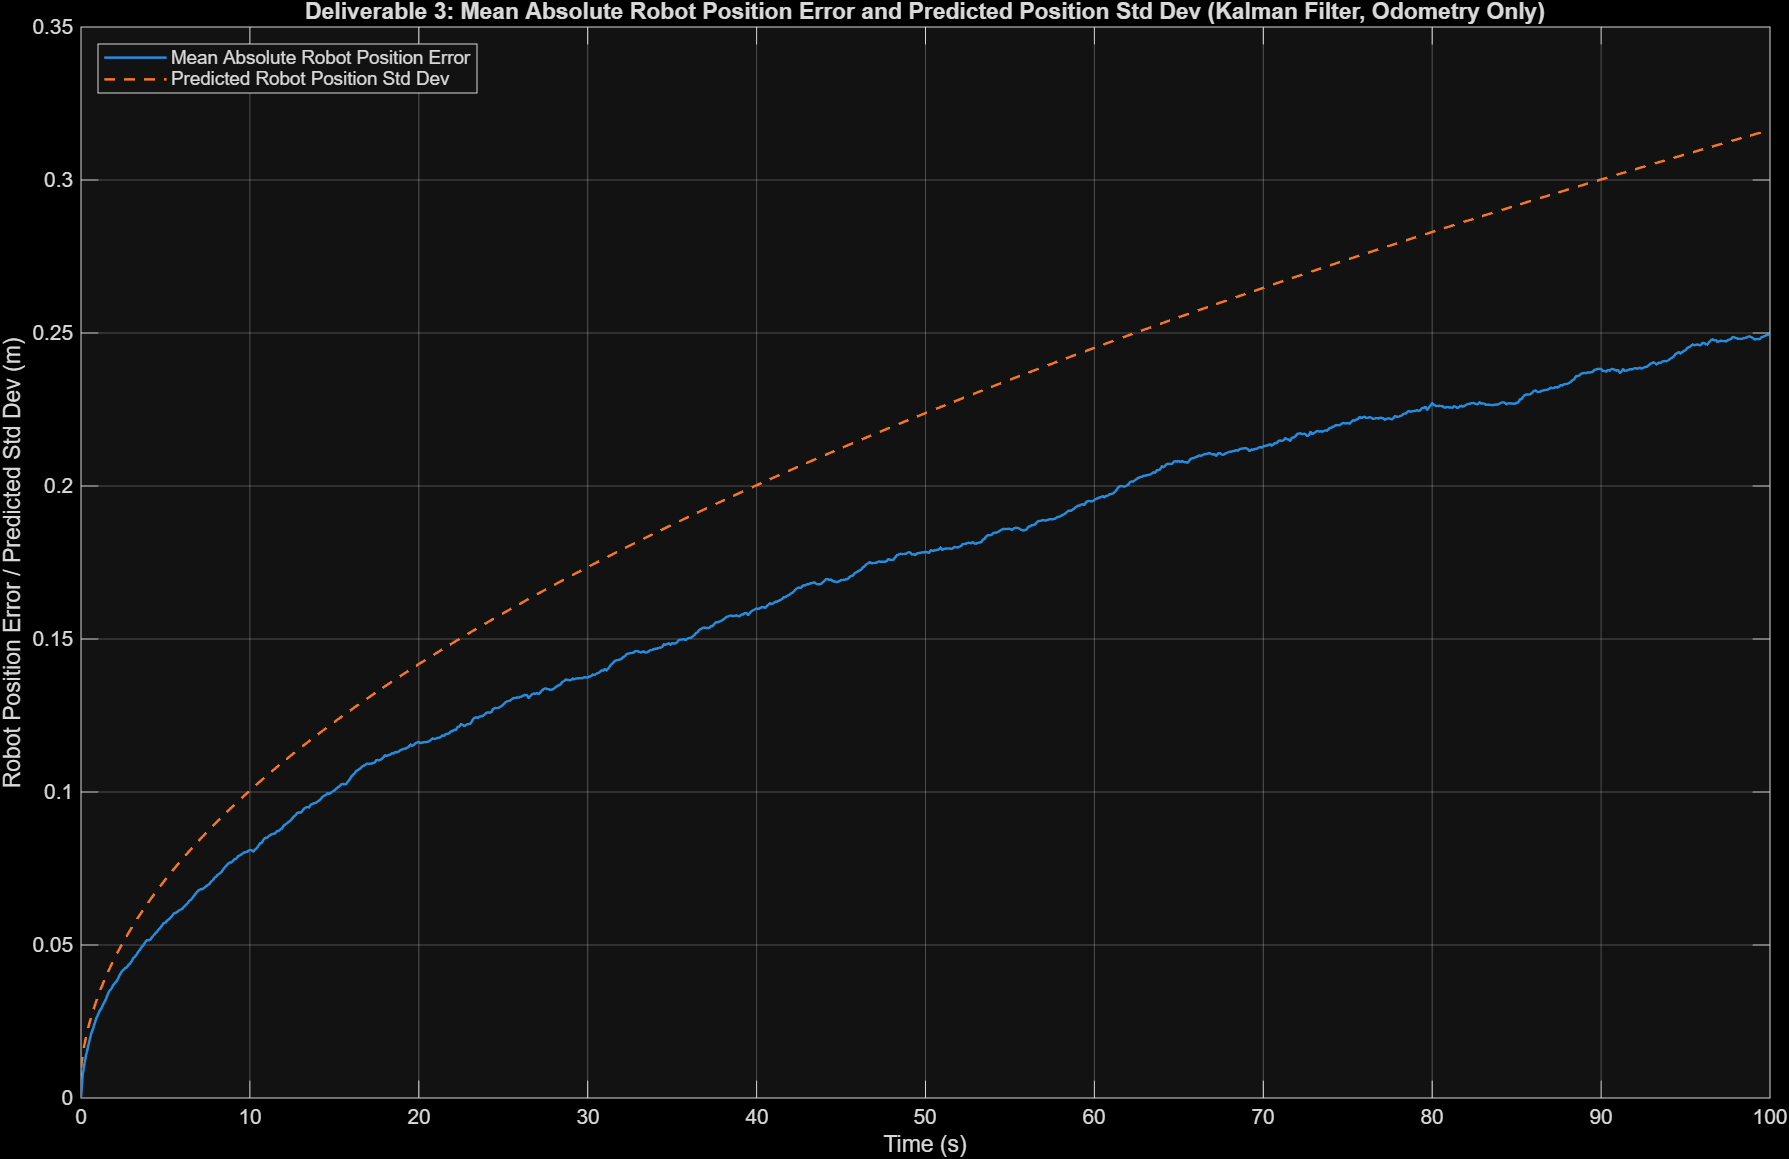
\includegraphics[width=0.9\textwidth]{Deliverable3.png}
\caption{Deliverable 3: Mean absolute robot position error and predicted position standard deviation for the odometry-only Kalman filter.}
\end{figure}

Compared with the first simulation (Least Squares Error - Odometry Only), the
odometry-only Kalman filter shows the same overall behavior: error grows over
time because the estimator relies only on noisy motion information and receives
no landmark-based correction - nothing to ground the robot back into the space
it is traversing. The main additional benefit of the Kalman filter
is that it also predicts its own uncertainty through $P_k$. In the plot, the
covariance-based position standard deviation increases with time in a manner 
that is consistent with the rising empirical error.

\section{Deliverable 4: Kalman Filter with Odometry and Landmark Sensing}
For simulation four, the Kalman filter was extended to use both odometry and landmark
measurements. The measurement matrix $H_k$ and noise covariance $R_k$ were allowed to
change dimension with time depending on which landmarks were within sensor range at each time
step.

\begin{figure}[H]
\centering
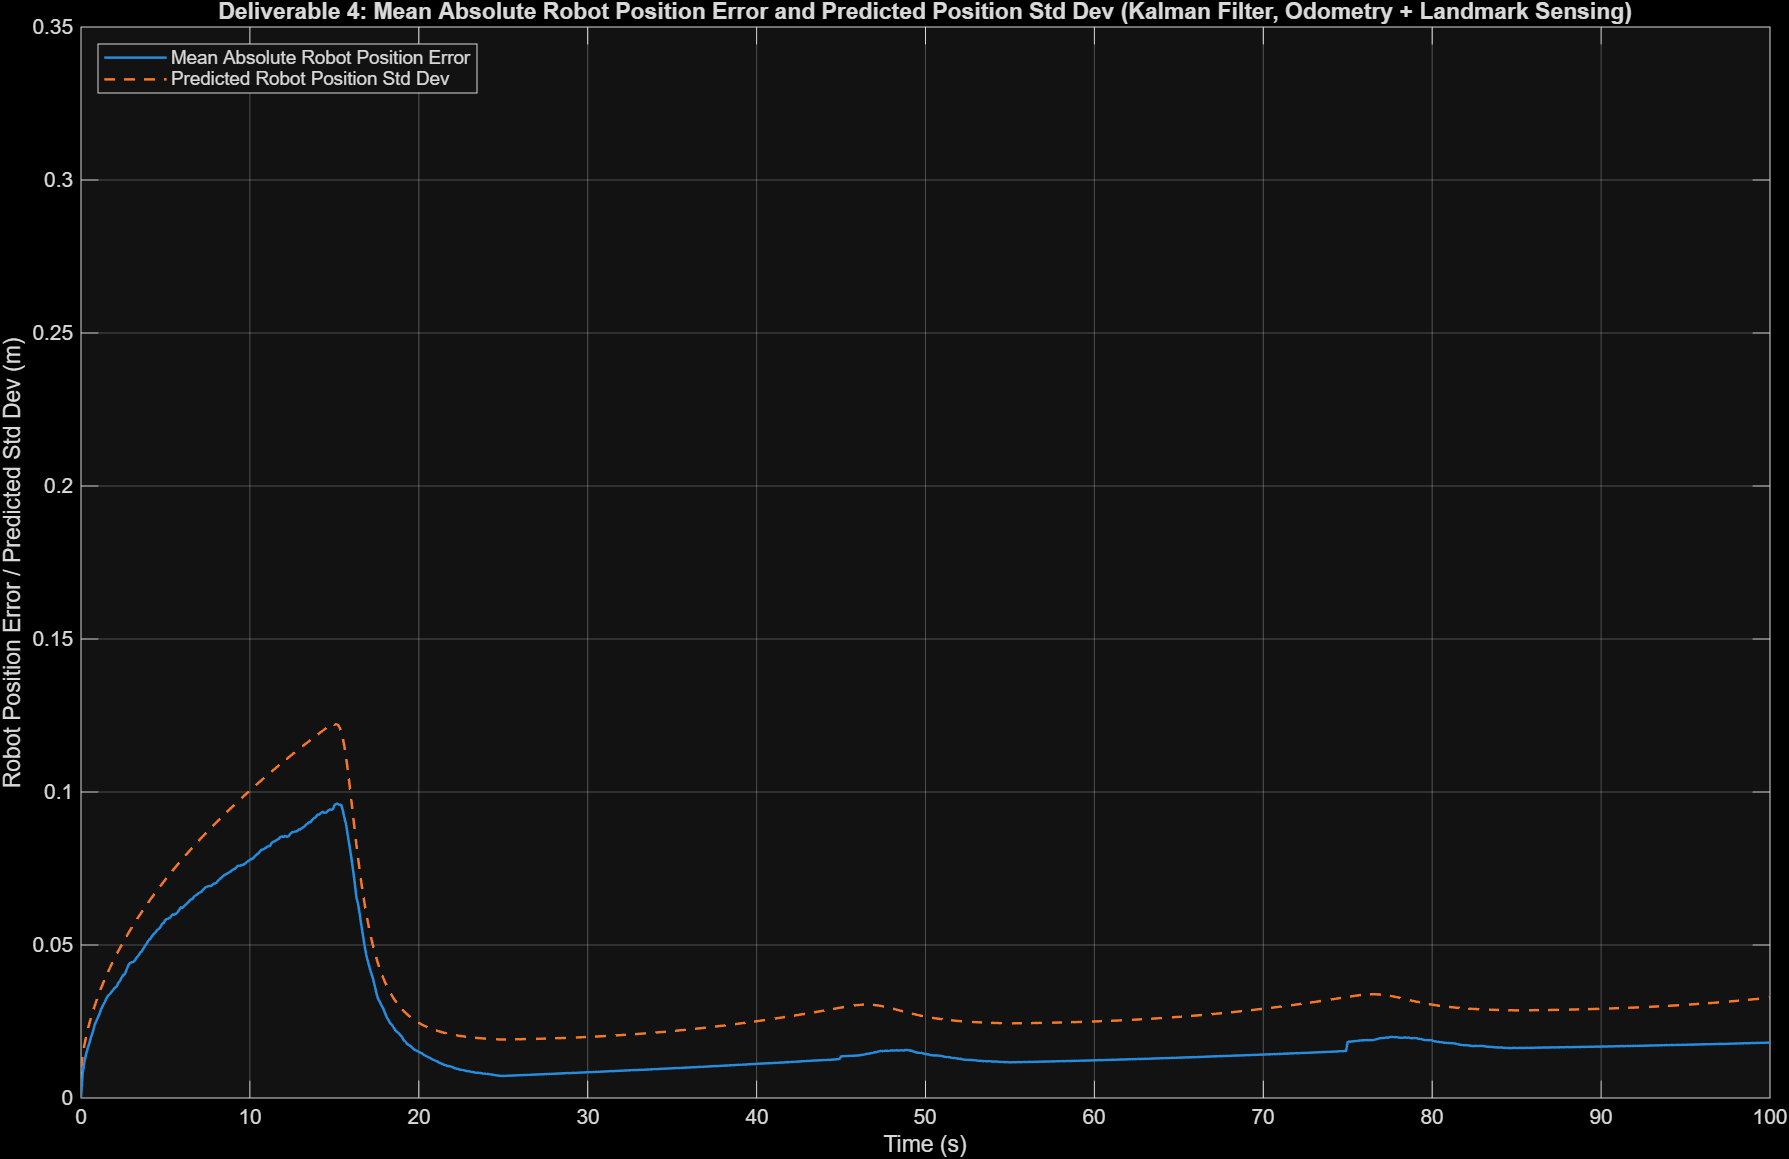
\includegraphics[width=0.9\textwidth]{Deliverable4.png}
\caption{Deliverable 4: Mean absolute robot position error and predicted position standard deviation for the Kalman filter with landmark sensing.}
\end{figure}

The robot's observation of landmarks clearly reduces the growth of error. Between
landmark sightings, the filter behaves similarly to the odometry-only case and
uncertainty gradually increases. This odometry-only-like behavior is most clear
before it sees a single landmark. When a landmark actually comes into range, the
extra measurement constrains the robot position and the predicted standard deviation
drops. The empirical mean absolute error also decreases or grows more slowly in those regions.

In the results obtained here, the Kalman filter also outperforms the corresponding batch
least squares result. Comparing simulation four with simulation two, the landmark-aware
Kalman filter maintains a substantially lower error level over the hallway traversal,
making it the strongest one-way estimator in these simulations.

Unlike the Kalman filter, which only uses the information available up to the current time step,
the batch least squares formulations with landmark sensing solve for the full trajectory and
landmark states simultaneously, so measurements from later times can influence earlier pose
estimates through the global solution. In spite of that, the Kalman filter produced
the lower error in these runs, while also providing a covariance-based uncertainty estimate
that the least squares plots do not directly provide.

\section{Deliverable 5: Batch Least Squares with Back-and-Forth Loop Closures}
For simulation five, the batch least squares formulation from simulation two was extended
so the robot traveled to the end of the hallway and then returned to the origin at
$-0.1$ m/s. This doubles the traversal duration and causes the robot to re-observe the
same landmarks on the return trip.

\begin{figure}[H]
\centering
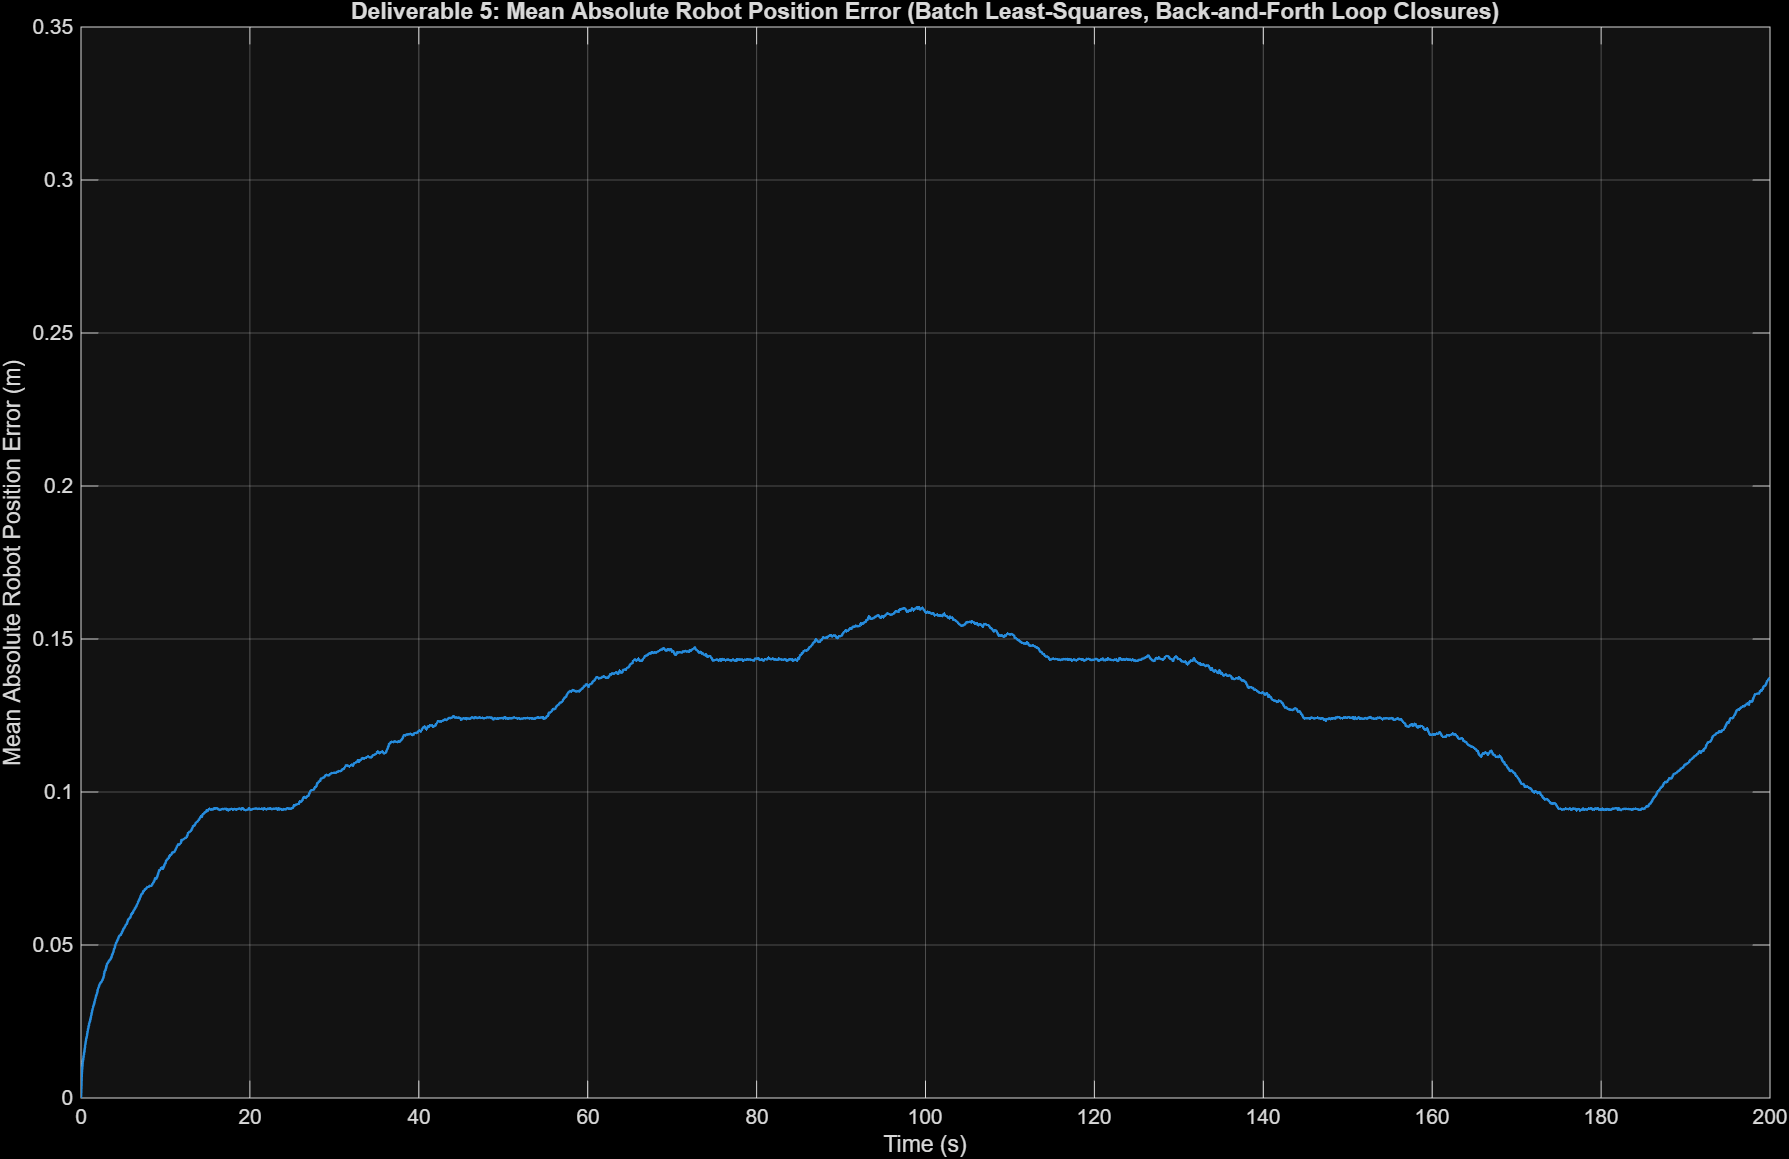
\includegraphics[width=0.9\textwidth]{Deliverable5.png}
\caption{Deliverable 5: Mean absolute robot position error for batch least squares with back-and-forth landmark re-observations.}
\end{figure}

The re-observation of landmarks does have a meaningful impact on the robot's ability to
curb the growth of error. These repeated landmark observations act as loop-closure
constraints: later robot poses are connected back to the same fixed landmark states
observed earlier in the run. As a result, accumulated drift is reduced on the return
trip, and the full back-and-forth trajectory estimate is better constrained than it
would be without those repeated observations.

\section{Conclusion}
Across all five simulations, the main pattern is consistent: odometry alone leads to
steadily increasing localization error, while landmark observations reduce drift by
anchoring the robot to fixed features in the hallway. In the results obtained during
these simulations, the Kalman filter outperformed the batch least squares approach
overall, with the landmark-aware Kalman filter in simulation four producing the lowest
sustained error among the one-way hallway traversals.

The back-and-forth batch least squares case in simulation five still demonstrates an
important SLAM effect: repeated landmark observations on the return trip help reduce
accumulated drift through loop-closure-style constraints. Even so, based on the plots
generated here, the Kalman filter produced the best overall localization performance in
this project while also providing an explicit covariance-based uncertainty estimate.

\section{Future Work}
If this work were extended beyond the guiding requirements, several next steps
would be valuable. First, implementing a return run for the Kalman filter would make it
possible to compare a back-and-forth recursive estimator directly against Deliverable 5
and study whether loop-closure-like repeated observations provide similar benefits in
the incremental setting. Second, the batch least squares implementations in simulation
one, two, and five could be refactored for readability, since the Kalman filter implementations
developed later in the assignment are more modular and easier to interpret at a glance.

Additional simulation studies would also help characterize estimator behavior more
deeply. Varying the number and placement of landmarks would show how map feature density
affects localization accuracy. Adjusting robot properties such as its speed and the
measurement update interval would also be useful, since changing the traversal speed or
the time-step would directly affect how quickly error accumulates and how often each
estimator receives information. Plotting the estimated state against the true state for
each variation would make the trajectory differences more visually interpretable than
error-only plots. Finally, extending the run time of each simulation would help evaluate
long-horizon error resilience and reveal how each method behaves when drift has more
time to accumulate.

\section{Included MATLAB Files}
The MATLAB source associated with this report is organized as follows:
\begin{itemize}[leftmargin=1.5em]
    \item \texttt{simlab1/sim.m}: driver script that runs all five deliverables and
    records summary notes
    \item \texttt{simlab1/sim1.m}: Deliverable 1 batch least squares implementation
    \item \texttt{simlab1/sim2.m}: Deliverable 2 batch least squares implementation
    with landmark sensing
    \item \texttt{simlab1/sim3.m}: Deliverable 3 odometry-only Kalman filter
    implementation
    \item \texttt{simlab1/sim4.m}: Deliverable 4 Kalman filter implementation with
    landmark sensing
    \item \texttt{simlab1/sim5.m}: Deliverable 5 back-and-forth batch least squares
    implementation
    \item \texttt{simlab1/problem\_setup\_orig.m}: provided starter setup file
\end{itemize}

\appendix
\section{MATLAB Source Code}

\subsection*{\texttt{sim.m}}
\begin{lstlisting}[caption={sim.m}, label={lst:simm}]
%{
% Author: Matthew Lepis
% Course: ME 656 - Autonomous Navigation for Mobile Robots
% Assignment: SimLab 1
% File: sim.m
%
% This driver script runs the simulations for:
%   sim1 -> Deliverable 1: odometry-only batch least-squares SLAM
%   sim2 -> Deliverable 2: batch least-squares SLAM with landmark sensing
%   sim3 -> Deliverable 3: odometry-only Kalman filter SLAM
%   sim4 -> Deliverable 4: Kalman filter SLAM with landmark sensing
%   sim5 -> Deliverable 5: batch least-squares SLAM with back-and-forth loop closures
%}

% Run Deliverable 1. This script estimates the robot trajectory using only
% odometry measurements and plots mean absolute pose error over time.
sim1

% Run Deliverable 2. This script adds landmark observations to the batch
% least-squares system and shows how landmarks reduce trajectory drift.
sim2

%
% Deliverable 2 shows that adding landmark observations slows the growth of
% localization error compared with Deliverable 1, which relied on odometry
% alone. In the odometry-only case, error tends to accumulate over time
% because each noisy motion measurement builds on the previous one without
% any external correction. With landmark measurements included, the robot
% periodically receives additional information that anchors its estimated
% position to fixed features in the hallway, which helps correct drift and
% reduces overall mean absolute error.
%
% As a result, the Deliverable 2 error curve should grow more slowly and
% remain lower than the Deliverable 1 curve, especially when the robot is
% within sensing range of landmarks. This demonstrates the core benefit of
% SLAM: map features do not just get estimated, they also improve
% localization accuracy by constraining the robot's trajectory.

% Run Deliverable 3. This script switches from batch least-squares to an
% incremental Kalman filter with odometry-only sensing and plots both the
% mean absolute position error and the filter-predicted position standard
% deviation over time.
sim3

%
% Deliverable 3 shows the same odometry-only drift behavior as Deliverable 1,
% but now through the lens of recursive state estimation. Because the Kalman
% filter only receives noisy velocity measurements and no landmark updates,
% its position estimate becomes progressively less certain as the robot moves
% down the hallway. That growing uncertainty appears both in the empirical
% mean absolute error curve and in the covariance-based standard deviation.
%
% Comparing these two curves is useful because it checks whether the filter's
% internal uncertainty estimate is consistent with what actually happens over
% many trials. In the odometry-only case, both curves should increase with
% time, reflecting the fact that motion noise accumulates when there is no
% external position correction.

% Run Deliverable 4. This script extends the Kalman filter to use both
% odometry and landmark measurements, and plots mean absolute position
% error alongside the filter-predicted position standard deviation.
sim4

%
% Deliverable 4 shows how landmark observations improve the recursive
% Kalman filter estimate. Between landmark sightings, the robot still
% accumulates odometry-driven uncertainty, so both error and predicted
% standard deviation tend to rise. When a landmark comes into range, the
% extra measurement constrains the robot position and the relevant
% uncertainty drops.
%
% Compared with Deliverable 3, the Deliverable 4 curves stay
% noticeably lower overall and show clear corrections around the landmark
% visibility windows. This highlights the same SLAM benefit seen in
% Deliverable 2, but now in an incremental filter setting rather than a
% batch least-squares solve.

% Run Deliverable 5. This script returns to the batch least-squares SLAM
% formulation, but now sends the robot to the end of the hallway and back
% to the origin so the same landmarks are re-observed on the return trip.
sim5

%
% Deliverable 5 highlights the impact of loop closures in batch least-
% squares SLAM. On the outbound trip, the robot accumulates odometry-driven
% drift much like Deliverable 2. On the return trip, however, it sees the
% same landmarks again, which adds new constraints that connect later robot
% poses back to the same fixed landmark states.
%
% Those repeated landmark observations reduce accumulated drift and
% improve the trajectory estimate over the full back-and-forth traversal.
% Compared with Deliverable 2, the Deliverable 5 mean absolute error curve
% shows the benefit of re-observing landmarks, especially after the
% robot turns around and begins revisiting previously seen hallway features.

\end{lstlisting}

\subsection*{\texttt{sim1.m}}
\begin{lstlisting}[caption={sim1.m}, label={lst:sim1}]
function sim1
length_hallway = 10;  % m
sensor_range = 0.5;  % m

landmarks = [2; 5; 8];  % m
num_landmarks = length(landmarks);  % 3

stdev_odometry = 0.1; % m/s
stdev_range = 0.01; % m

%%%%%%%%%%%%%%%%%%%%%%%%%%%%%%%%%%%%%%%%%%%%%%%%%%%%%%%%%%%%%%%%%%%
% Robot ground-truth trajectory for the hallway traversal
%%%%%%%%%%%%%%%%%%%%%%%%%%%%%%%%%%%%%%%%%%%%%%%%%%%%%%%%%%%%%%%%%%%

delta_t = 0.1; % time is discretized with a time-step of 0.1 seconds
v_robot = 0.1; % robot travels at a constant speed of 0.1 m/s

t_terminal = length_hallway/v_robot; % time that we reach the end of hall

t_vector = 0:delta_t:t_terminal; % time vector for robot's trajectory
x_vector = 0:v_robot*delta_t:length_hallway; % true robot position over time
v_vector = ones(1,length(t_vector)).*v_robot;  % true robot velocity over time

num_states = length(x_vector); % number of discrete-time pose states

% Batch least-squares state:
%   [x_0, x_1, ..., x_K]^T
%
% Odometry rows encode consecutive pose differences:
%   x_k - x_(k-1) = z_odom(k)
% where z_odom(k) = (v_k + noise) * delta_t.
%
% Row 1 is the special initial-condition constraint x_0 = 0.

%% Deliverable 1: Batch Least-Squares SLAM with Odometry-Only Measurements
num_of_trials = 1000;

% Build the matching linear measurement matrix.
A_matrix = zeros(num_states, num_states);
A_matrix(1,1) = 1;  % Special initial-condition row: x_0 = 0
for k = 2:num_states
    A_matrix(k, k-1) = -1;
    A_matrix(k, k) = 1;
end

abs_error = zeros(num_of_trials, num_states);
for trial = 1:num_of_trials
    % Build the measurement vector with the initial condition and odometry.
    b_vector = zeros(num_states, 1);
    b_vector(1) = 0;
    for k = 2:num_states
        meas_noise = stdev_odometry * randn();
        b_vector(k) = (v_vector(k) + meas_noise) * delta_t;
    end

    % Solve for the full robot trajectory in one batch.
    x_estimates = A_matrix \ b_vector;

    % Store this trial's absolute pose error over time.
    abs_error(trial, :) = abs(x_estimates - x_vector(:)).';
end

mean_state_abs_error = mean(abs_error, 1);
figure;
plot(t_vector, mean_state_abs_error, 'LineWidth', 1.8)
xlabel('Time (s)')
ylabel('Mean Absolute Robot Position Error (m)')
title('Deliverable 1: Mean Absolute Robot Position Error (Batch Least-Squares, Odometry Only)')
ylim([0, 0.35])
grid on

%{
%%% Deliverable 1: Supplemental Plots

% Plot noisy odometry displacement measurements for one trial.
%
% figure;
% plot(t_vector(2:end), b_vector(2:end))
% ylabel('Measured displacement per step (m)')
% xlabel('Time (s)')
% title('Noisy odometry displacement measurements')
% ylim([0, 0.35])
grid on

% odom_measurement_mean = mean(b_vector(2:end)); % Should be ~0.01
% odom_measurement_std = std(b_vector(2:end));   % Should be ~0.01

% Plot true vs estimated robot position for one trial.
%
% figure;
% plot(t_vector, x_vector, 'LineWidth', 4)
% hold on
% plot(t_vector, x_estimates, ':', 'LineWidth', 2)
% xlabel('Time (s)')
% ylabel('Position (m)')
% title('True vs Estimated Robot Position (Odometry Only)')
% legend('True Position', 'Estimated Position')
% ylim([0, 0.35])
grid on

% Plot single-trial absolute position error over time.
%
% figure;
% plot(t_vector, abs_error(1, :), 'LineWidth', 1.2)
% xlabel('Time (s)')
% ylabel('Absolute Position Error (m)')
% title('Absolute Position Error Over Time')
% ylim([0, 0.35])
grid on
%}
end

\end{lstlisting}

\subsection*{\texttt{sim2.m}}
\begin{lstlisting}[caption={sim2.m}, label={lst:sim2}]
function sim2
length_hallway = 10;  % m
sensor_range = 0.5;  % m

landmarks = [2; 5; 8];  % m
num_landmarks = length(landmarks);  % 3

stdev_odometry = 0.1; % m/s
stdev_range = 0.01; % m

%%%%%%%%%%%%%%%%%%%%%%%%%%%%%%%%%%%%%%%%%%%%%%%%%%%%%%%%%%%%%%%%%%%
% Robot ground-truth trajectory for the hallway traversal
%%%%%%%%%%%%%%%%%%%%%%%%%%%%%%%%%%%%%%%%%%%%%%%%%%%%%%%%%%%%%%%%%%%

delta_t = 0.1; % time is discretized with a time-step of 0.1 seconds
v_robot = 0.1; % robot travels at a constant speed of 0.1 m/s

t_terminal = length_hallway / v_robot; % time that we reach the end of hall

t_vector = 0:delta_t:t_terminal; % time vector for robot's trajectory
x_vector = 0:v_robot*delta_t:length_hallway; % true robot position over time
v_vector = ones(1, length(t_vector)) .* v_robot; % true robot velocity over time

num_states = length(x_vector); % number of discrete-time pose states

% Batch least-squares state:
%   [x_0, x_1, ..., x_K, l_1, l_2, l_3]^T
%
% Odometry rows encode consecutive pose differences:
%   x_k - x_(k-1) = z_odom(k)
% where z_odom(k) = (v_k + noise) * delta_t.
%
% Landmark rows encode signed robot-to-landmark displacement:
%   l_j - x_k = z_range(k,j)
% This keeps the landmark measurement model linear in the unknown states.
%
% Row 1 is the special initial-condition constraint x_0 = 0.

function measurement = odometryMeasurement(time_step)
    odo_noise = stdev_odometry * randn();
    measurement = (v_vector(time_step) + odo_noise) * delta_t;
end

function in_range = inRange(time_step, true_landmark_pose)
    if abs(true_landmark_pose - x_vector(time_step)) <= sensor_range
        in_range = true;
    else
        in_range = false;
    end
end

function measurements = sensorMeasurements(time_step)
    measurements = zeros(num_landmarks, 1);
    for landmark = 1:num_landmarks
        true_landmark_pose = landmarks(landmark);

        if inRange(time_step, true_landmark_pose)
            true_robot_pose = x_vector(time_step);
            range_sensor_noise = stdev_range * randn();

            % Signed displacement keeps the batch system linear.
            noisy_range_to_landmark = true_landmark_pose - true_robot_pose + range_sensor_noise;
            measurements(landmark) = noisy_range_to_landmark;
        else
            % Placeholder row; removed before solving.
            measurements(landmark) = nan;
        end
    end
end

function b_vector = bStorageHandling(b_vector, time_step)
    % Landmark measurements for one time-step occupy a contiguous block
    % after the odometry rows.
    idx_shift = num_states + (time_step - 1) * num_landmarks;

    sensor_measurements = sensorMeasurements(time_step);
    for landmark = 1:num_landmarks
        b_vector(idx_shift + landmark) = sensor_measurements(landmark);
    end
end

function A_matrix = AStorageHandling(A_matrix, time_step)
    % Each landmark row encodes l_j - x_k = z_range(k,j).
    idx_shift = num_states + (time_step - 1) * num_landmarks;

    for landmark = 1:num_landmarks
        row = idx_shift + landmark;
        A_matrix(row, time_step) = -1;
        A_matrix(row, num_states + landmark) = 1;
    end
end

%% Deliverable 2: Batch Least-Squares SLAM with Odometry + Landmark Measurements
num_of_trials = 1000;

% Build the matching linear measurement matrix.
A_matrix = zeros(num_states + num_landmarks * num_states, num_states + num_landmarks);
A_matrix(1, 1) = 1;  % Special initial-condition row: x_0 = 0
A_matrix = AStorageHandling(A_matrix, 1);

for k = 2:num_states
    A_matrix(k, k-1) = -1;
    A_matrix(k, k) = 1;
    A_matrix = AStorageHandling(A_matrix, k);
end

t0 = tic;
h = waitbar(0, 'Starting...');
cleanupObj = onCleanup(@() close(h));

state_abs_error = zeros(num_of_trials, num_states + num_landmarks);
landmark_estimate_history = zeros(num_of_trials, num_landmarks);
for trial = 1:num_of_trials
    % Build the measurement vector: initial condition, odometry, then
    % in-range landmark observations.
    num_pose_landmark_states = num_states + num_landmarks * num_states;
    b_vector = zeros(num_pose_landmark_states, 1);

    b_vector(1) = 0;
    b_vector = bStorageHandling(b_vector, 1);

    for time_step = 2:num_states
        b_vector(time_step) = odometryMeasurement(time_step);
        b_vector = bStorageHandling(b_vector, time_step);
    end

    % Remove placeholder rows for landmarks that were out of range.
    valid_rows = ~isnan(b_vector);
    b_valid = b_vector(valid_rows);
    if trial == 1
        A_valid = A_matrix(valid_rows, :);
    end

    % Solve for all robot poses and landmark locations in one batch.
    state_estimates = A_valid \ b_valid;
    landmark_estimates = state_estimates(num_states + 1:end);
    landmark_estimate_history(trial, :) = landmark_estimates.';

    state_truth = [x_vector(:); landmarks(:)];
    state_abs_error(trial, :) = abs(state_estimates - state_truth).';

    if mod(trial, 25) == 0 || trial == 1 || trial == num_of_trials
        elapsed = toc(t0);
        eta = elapsed * (num_of_trials - trial) / trial;
        msg = sprintf('Progress: %d/%d | ETA: %.1f s', trial, num_of_trials, eta);
        waitbar(trial / num_of_trials, h, msg);
    end

end

mean_state_abs_error = mean(state_abs_error, 1);
mean_landmark_estimates = mean(landmark_estimate_history, 1).';
mean_pose_abs_error = mean_state_abs_error(1:num_states);
mean_landmark_abs_error = mean_state_abs_error(num_states + 1:end);

figure;
plot(t_vector, mean_pose_abs_error, 'LineWidth', 1.2)
xlabel('Time (s)')
ylabel('Mean Absolute Robot Position Error (m)')
title('Deliverable 2: Mean Absolute Robot Position Error (Batch Least-Squares, Odometry + Landmark Sensing)')
ylim([0, 0.35])
grid on

disp(table((1:num_landmarks).', landmarks, mean_landmark_estimates, mean_landmark_abs_error(:), ...
    'VariableNames', {'Landmark', 'Truth', 'MeanEstimate', 'MeanAbsError'}))
end
\end{lstlisting}

\subsection*{\texttt{sim3.m}}
\begin{lstlisting}[caption={sim3.m}, label={lst:sim3}]
function sim3
length_hallway = 10;  % m
sensor_range = 0.5;  % m

landmarks = [2; 5; 8];  % m
num_landmarks = length(landmarks);  % 3

stdev_odometry = 0.1; % m/s
stdev_range = 0.01; % m

%%%%%%%%%%%%%%%%%%%%%%%%%%%%%%%%%%%%%%%%%%%%%%%%%%%%%%%%%%%%%%%%%%%
% Robot ground-truth trajectory for the hallway traversal
%%%%%%%%%%%%%%%%%%%%%%%%%%%%%%%%%%%%%%%%%%%%%%%%%%%%%%%%%%%%%%%%%%%

delta_t = 0.1; % time is discretized with a time-step of 0.1 seconds
v_robot = 0.1; % robot travels at a constant speed of 0.1 m/s

t_terminal = length_hallway/v_robot; % time that we reach the end of hall

t_vector = 0:delta_t:t_terminal; % time vector for robot's trajectory
x_vector = 0:v_robot*delta_t:length_hallway; % true robot position over time
v_vector = ones(1,length(t_vector)).*v_robot;  % true robot velocity over time

num_states = length(x_vector); % number of discrete-time pose states

% Kalman filter state:
%   [v_k, x_k, l_1, l_2, l_3]^T
%
% Process model:
%   X_(k+1) = A * X_k + w_k
% where the robot keeps a constant velocity and the landmarks remain static.
%
% Deliverable 3 uses odometry-only updates:
%   z_k = H * X_k + n_k
% with H = [1 0 0 0 0], so odometry is modeled as a direct noisy
% measurement of the velocity state.
%
% The initial covariance reflects:
%   var(v_0) = 1
%   var(x_0) = 0.0001
%   var(l_j) = 1
%
% Landmark states stay in the vector for consistency with later
% deliverables, but they are not observed in this odometry-only case.

Q_11 = 1e-8;

velocity_variance = 1;
position_variance = 1e-4;
landmark_1_variance = 1;
landmark_2_variance = 1;
landmark_3_variance = 1;

P_0 = ...
    [
    velocity_variance, 0, 0, 0, 0;
    0, position_variance, 0, 0, 0;
    0, 0, landmark_1_variance, 0, 0;
    0, 0, 0, landmark_2_variance, 0;
    0, 0, 0, 0, landmark_3_variance
    ];

x_0 = [ v_robot;    0;  0;  0;  0; ];

A = [ 1, 0, 0, 0, 0;    delta_t, 1, 0, 0, 0;    0, 0, 1, 0, 0;      0, 0, 0, 1, 0;      0, 0, 0, 0, 1 ];

Q = [ Q_11, 0, 0, 0, 0; 0, 0, 0, 0, 0;          0, 0, 0, 0, 0;      0, 0, 0, 0, 0;      0, 0, 0, 0, 0 ];

    function H = genH()
        % Odometry is a direct noisy measurement of the velocity state.
        % State ordering: [velocity; position; l1; l2; l3]
        H = [1, 0, 0, 0, 0];
    end

    function R = genR()
        % Scalar odometry measurement noise covariance.
        R = stdev_odometry^2;
    end

    function [x_k_predict, P_k_predict] = predict(x_k_last, P_k_last)
        % Time update: propagate the state estimate and its covariance.
        x_k_predict = A * x_k_last;
        P_k_predict = A * P_k_last * A' + Q;
    end

    function [x_k, P_k] = correct(x_k_predict, P_k_predict, z_k, H, R)
        % Measurement update with the current odometry reading.
        H_T = transpose(H);

        K_k = P_k_predict * H_T / (H * P_k_predict * H_T + R);

        x_k = x_k_predict + K_k * (z_k - H * x_k_predict);
        P_k = (eye(5,5) - K_k * H) * P_k_predict;
    end

    function velocity_meas = odometryMeasurement(time_step)
        % Simulate one noisy odometry velocity measurement.
        odo_noise = stdev_odometry * randn();
        velocity_meas = (v_vector(time_step) + odo_noise);
    end

    function z_k = gatherMeasurements(time_step)
        % Build the measurement vector for one time-step.
        % Deliverable 3 uses odometry only, so the landmark entries are
        % placeholders that get removed before the correction step.
        velocity_meas = odometryMeasurement(time_step);
        position_meas = nan;  % Odometry only, no position
        landmark1_meas = nan;  % Odometry only, no range sensing to Landmark 1
        landmark2_meas = nan;  % Odometry only, no range sensing to Landmark 2
        landmark3_meas = nan;  % Odometry only, no range sensing to Landmark 3

        z_k = [
            velocity_meas;
            position_meas;
            landmark1_meas;
            landmark2_meas;
            landmark3_meas;
            ];
        valid_rows = ~isnan(z_k);
        z_k = z_k(valid_rows);
    end

%% Deliverable 3: Odometry-Only Kalman Filter
num_of_trials = 1000;

std_position_error = zeros(1, num_states);
estimated_position = zeros(num_of_trials, num_states);
for trial = 1:num_of_trials
    % k = 1, aka t=0
    x_k_last = x_0;
    P_k_last = P_0;
    estimated_position(trial, 1) = x_0(2);
    if trial == 1
        % P evolution is deterministic here, so one trial is sufficient for the sigma curve.
        std_position_error(1) = sqrt(P_0(2,2));
    end
    for k = 2:num_states
        % Step 1: Predict
        [x_k_predict, P_k_predict] = predict(x_k_last, P_k_last);

        % Step 2: Correct
        z_k = gatherMeasurements(k);
        H = genH();
        R = genR();
        [x_k, P_k] = correct(x_k_predict, P_k_predict, z_k, H, R);

        x_k_last = x_k;
        P_k_last = P_k;
        estimated_position(trial, k) = x_k(2);
        if trial == 1
            % P evolution is deterministic here, so one trial is sufficient for the sigma curve.
            std_position_error(k) = sqrt(P_k(2,2));
        end
    end
end

% Compare each trial's estimated trajectory against the ground-truth hallway motion.
trial_abs_position_error = abs(estimated_position - x_vector).';
mean_trial_abs_position_error = mean(trial_abs_position_error, 2);

% Plot the Monte Carlo mean absolute error and the covariance-predicted
% position standard deviation on the same axes.
figure; 
plot(t_vector, mean_trial_abs_position_error, 'LineWidth', 1.2)
hold on
plot(t_vector, std_position_error, '--', 'LineWidth', 1.2)
xlabel('Time (s)')
ylabel('Robot Position Error / Predicted Std Dev (m)')
title('Deliverable 3: Mean Absolute Robot Position Error and Predicted Position Std Dev (Kalman Filter, Odometry Only)')
legend('Mean Absolute Robot Position Error', 'Predicted Robot Position Std Dev', 'Location', 'northwest')
ylim([0, 0.35])
grid on
end

\end{lstlisting}

\subsection*{\texttt{sim4.m}}
\begin{lstlisting}[caption={sim4.m}, label={lst:sim4}]
function sim4
length_hallway = 10;  % m
sensor_range = 0.5;  % m

landmarks = [2; 5; 8];  % m
num_landmarks = length(landmarks);  % 3

stdev_odometry = 0.1; % m/s
stdev_range = 0.01; % m

%%%%%%%%%%%%%%%%%%%%%%%%%%%%%%%%%%%%%%%%%%%%%%%%%%%%%%%%%%%%%%%%%%%
% Robot ground-truth trajectory for the hallway traversal
%%%%%%%%%%%%%%%%%%%%%%%%%%%%%%%%%%%%%%%%%%%%%%%%%%%%%%%%%%%%%%%%%%%

delta_t = 0.1; % time is discretized with a time-step of 0.1 seconds
v_robot = 0.1; % robot travels at a constant speed of 0.1 m/s

t_terminal = length_hallway/v_robot; % time that we reach the end of hall

t_vector = 0:delta_t:t_terminal; % time vector for robot's trajectory
x_vector = 0:v_robot*delta_t:length_hallway; % true robot position over time
v_vector = ones(1,length(t_vector)).*v_robot;  % true robot velocity over time

num_states = length(x_vector); % number of discrete-time pose states

% Kalman filter state:
%   [v_k, x_k, l_1, l_2, l_3]^T
%
% Process model:
%   X_(k+1) = A * X_k + w_k
% where the robot keeps a constant velocity and the landmarks remain static.
%
% Deliverable 4 uses both odometry and landmark updates:
%   z_k = H_k * X_k + n_k
% The measurement model changes size with time because the robot always
% receives one odometry measurement, and may also receive one or more
% landmark range measurements whenever landmarks fall within sensor range.
%
% Odometry is modeled as a direct noisy measurement of the velocity state.
% Landmark range measurements are modeled as signed displacement:
%   l_j - x_k + noise
% which keeps the measurement model linear in the unknown states.
%
% The initial covariance reflects:
%   var(v_0) = 1
%   var(x_0) = 0.0001
%   var(l_j) = 1

Q_11 = 1e-8;

velocity_variance = 1;
position_variance = 1e-4;
landmark_1_variance = 1;
landmark_2_variance = 1;
landmark_3_variance = 1;

P_0 = ...
    [
    velocity_variance, 0, 0, 0, 0;
    0, position_variance, 0, 0, 0;
    0, 0, landmark_1_variance, 0, 0;
    0, 0, 0, landmark_2_variance, 0;
    0, 0, 0, 0, landmark_3_variance
    ];

x_0 = [ v_robot;    0;  0;  0;  0; ];

A = [ 1, 0, 0, 0, 0;    delta_t, 1, 0, 0, 0;    0, 0, 1, 0, 0;      0, 0, 0, 1, 0;      0, 0, 0, 0, 1 ];

Q = [ Q_11, 0, 0, 0, 0; 0, 0, 0, 0, 0;          0, 0, 0, 0, 0;      0, 0, 0, 0, 0;      0, 0, 0, 0, 0 ];

    function in_range = inRange(time_step, true_landmark_pose)
        % Return whether the robot can sense this landmark at the current time-step.
        if abs(true_landmark_pose - x_vector(time_step)) <= sensor_range
            in_range = true;
        else
            in_range = false;
        end
    end

    function landmarks_in_range = whichInRange(time_step)
        % Collect the indices of all landmarks that are visible right now.
        landmarks_in_range = [];
        for landmark = 1:num_landmarks
            true_landmark_pose = landmarks(landmark);
  
            if inRange(time_step, true_landmark_pose)
                landmarks_in_range = [landmarks_in_range, landmark];
            end       
        end
    end

    function H = genH(time_step)
        % Build the time-varying measurement matrix.
        % Row 1 is odometry, and each additional row encodes:
        %   l_j - x_k = z_range(k,j)
        in_range_landmarks = whichInRange(time_step);

        H = [1, 0, 0, 0, 0];
        for landmark = in_range_landmarks
            row = zeros(1, 5);
            row(2) = -1;
            row(landmark + 2) = 1;   % landmark 1 -> col 3, 2 -> col 4, 3 -> col 5
            H = [H; row];
        end
    end

    function R = genR(time_step)
        % Build the time-varying diagonal sensor covariance matrix.
        % Odometry is always present; each visible landmark adds one
        % independent range variance on the diagonal.
        in_range_landmarks = whichInRange(time_step);
        
        variances = stdev_odometry^2;
        for landmark = in_range_landmarks
            variances = [variances, stdev_range^2];
        end
        R = diag(variances);
    end

    function [x_k_predict, P_k_predict] = predict(x_k_last, P_k_last)
        % Time update: propagate the state estimate and its covariance.
        x_k_predict = A * x_k_last;
        P_k_predict = A * P_k_last * A' + Q;
    end

    function [x_k, P_k] = correct(x_k_predict, P_k_predict, z_k, H, R)
        % Measurement update with the current odometry and landmark readings.
        H_T = transpose(H);

        K_k = P_k_predict * H_T / (H * P_k_predict * H_T + R);

        x_k = x_k_predict + K_k * (z_k - H * x_k_predict);
        P_k = (eye(5,5) - K_k * H) * P_k_predict;
    end

    function velocity_meas = odometryMeasurement(time_step)
        % Simulate one noisy odometry velocity measurement.
        odo_noise = stdev_odometry * randn();
        velocity_meas = (v_vector(time_step) + odo_noise);
    end

    function [landmark1_meas, landmark2_meas, landmark3_meas] = landmarkMeasurements(time_step)
        % Simulate signed range measurements for any landmarks currently in range.
        measurements = nan(1, num_landmarks);
        for landmark = 1:num_landmarks
            true_landmark_pose = landmarks(landmark);

            if inRange(time_step, true_landmark_pose)
                true_robot_pose = x_vector(time_step);
                range_sensor_noise = stdev_range * randn();

                % Signed displacement keeps the Kalman measurement model linear.
                noisy_range_to_landmark = true_landmark_pose - true_robot_pose + range_sensor_noise;
                measurements(landmark) = noisy_range_to_landmark;
            end
        end
        tmp = num2cell(measurements);
        [landmark1_meas, landmark2_meas, landmark3_meas] = tmp{:};
    end

    function z_k = gatherMeasurements(time_step)
        % Build the measurement vector for one time-step.
        % Deliverable 4 uses odometry and landmark sensing.
        velocity_meas = odometryMeasurement(time_step);
        position_meas = nan;  % No direct position measurement
        [landmark1_meas, landmark2_meas, landmark3_meas] = landmarkMeasurements(time_step);

        z_k = [
            velocity_meas;
            position_meas;
            landmark1_meas;
            landmark2_meas;
            landmark3_meas;
            ];
        valid_rows = ~isnan(z_k);
        z_k = z_k(valid_rows);
    end

%% Deliverable 4: Kalman Filter with Odometry + Landmark Measurements
num_of_trials = 1000;

std_position_error = zeros(1, num_states);
estimated_position = zeros(num_of_trials, num_states);
for trial = 1:num_of_trials
    % k = 1, aka t=0
    x_k_last = x_0;
    P_k_last = P_0;
    estimated_position(trial, 1) = x_0(2);
    if trial == 1
        % P evolution is deterministic here, so one trial is sufficient for the sigma curve.
        std_position_error(1) = sqrt(P_0(2,2));
    end
    for k = 2:num_states
        % Step 1: Predict
        [x_k_predict, P_k_predict] = predict(x_k_last, P_k_last);

        % Step 2: Correct using the available measurements at this time-step.
        z_k = gatherMeasurements(k);
        H = genH(k);
        R = genR(k);
        [x_k, P_k] = correct(x_k_predict, P_k_predict, z_k, H, R);

        x_k_last = x_k;
        P_k_last = P_k;
        estimated_position(trial, k) = x_k(2);
        if trial == 1
            % P evolution is deterministic here, so one trial is sufficient for the sigma curve.
            std_position_error(k) = sqrt(P_k(2,2));
        end
    end
end

% Compare each trial's estimated trajectory against the ground-truth hallway motion.
trial_abs_position_error = abs(estimated_position - x_vector).';
mean_trial_abs_position_error = mean(trial_abs_position_error, 2);

% Plot the Monte Carlo mean absolute error and the covariance-predicted
% position standard deviation on the same axes.
figure; 
plot(t_vector, mean_trial_abs_position_error, 'LineWidth', 1.2)
hold on
plot(t_vector, std_position_error, '--', 'LineWidth', 1.2)
xlabel('Time (s)')
ylabel('Robot Position Error / Predicted Std Dev (m)')
title('Deliverable 4: Mean Absolute Robot Position Error and Predicted Position Std Dev (Kalman Filter, Odometry + Landmark Sensing)')
legend('Mean Absolute Robot Position Error', 'Predicted Robot Position Std Dev', 'Location', 'northwest')
ylim([0, 0.35])
grid on
end

\end{lstlisting}

\subsection*{\texttt{sim5.m}}
\begin{lstlisting}[caption={sim5.m}, label={lst:sim5}]
function sim5
length_hallway = 10;  % m
sensor_range = 0.5;  % m

landmarks = [2; 5; 8];  % m
num_landmarks = length(landmarks);  % 3

stdev_odometry = 0.1; % m/s
stdev_range = 0.01; % m

%%%%%%%%%%%%%%%%%%%%%%%%%%%%%%%%%%%%%%%%%%%%%%%%%%%%%%%%%%%%%%%%%%%
% Robot ground-truth trajectory for the back-and-forth hallway traversal
%%%%%%%%%%%%%%%%%%%%%%%%%%%%%%%%%%%%%%%%%%%%%%%%%%%%%%%%%%%%%%%%%%%
delta_t = 0.1; % time is discretized with a time-step of 0.1 seconds
v_robot = 0.1; % robot travels toward the end of the hallway at 0.1 m/s
v_robot_rev = -0.1; % robot returns to the origin at -0.1 m/s

t_terminal = length_hallway / v_robot; % time when the robot first reaches the end of hall
t_terminal_rev = -length_hallway / v_robot_rev; % time needed to return to the origin
t_terminal_total = t_terminal + t_terminal_rev;

t_vector = 0:delta_t:t_terminal; % forward-leg time vector
t_vector_rev = t_terminal+delta_t:delta_t:t_terminal_total; % return-leg time vector
t_vector_total = [t_vector, t_vector_rev];

x_vector = 0:v_robot*delta_t:length_hallway; % forward-leg ground-truth positions
x_vector_rev = length_hallway+v_robot_rev*delta_t:v_robot_rev*delta_t:0; % return-leg ground-truth positions
x_vector_total = [x_vector, x_vector_rev];

v_vector = ones(1, length(t_vector)) .* v_robot; % forward-leg velocity history
v_vector_rev = ones(1, length(t_vector_rev)) .* v_robot_rev; % return-leg velocity history
v_vector_total = [v_vector, v_vector_rev];

num_states = length(x_vector_total); % number of discrete-time pose states

% Batch least-squares state:
%   [x_0, x_1, ..., x_K, l_1, l_2, l_3]^T
%
% Odometry rows encode consecutive pose differences:
%   x_k - x_(k-1) = z_odom(k)
% where z_odom(k) = (v_k + noise) * delta_t.
%
% Landmark rows encode signed robot-to-landmark displacement:
%   l_j - x_k = z_range(k,j)
% This keeps the landmark measurement model linear in the unknown states.
%
% Deliverable 5 extends Deliverable 2 by sending the robot to the end of
% the hallway and then back to the origin. Re-observing the same landmarks
% on the return trip creates loop-closure constraints in the batch system.
%
% Row 1 is the special initial-condition constraint x_0 = 0.

function measurement = odometryMeasurement(time_step)
    % Simulate one noisy odometry displacement measurement.
    odo_noise = stdev_odometry * randn();
    measurement = (v_vector_total(time_step) + odo_noise) * delta_t;
end

function in_range = inRange(time_step, true_landmark_pose)
    % Return whether the robot can sense this landmark at the current time-step.
    if abs(true_landmark_pose - x_vector_total(time_step)) <= sensor_range
        in_range = true;
    else
        in_range = false;
    end
end

function measurements = sensorMeasurements(time_step)
    % Simulate signed landmark measurements for all landmarks currently in range.
    measurements = zeros(num_landmarks, 1);
    for landmark = 1:num_landmarks
        true_landmark_pose = landmarks(landmark);

        if inRange(time_step, true_landmark_pose)
            true_robot_pose = x_vector_total(time_step);
            range_sensor_noise = stdev_range * randn();

            % Signed displacement keeps the batch system linear.
            noisy_range_to_landmark = true_landmark_pose - true_robot_pose + range_sensor_noise;
            measurements(landmark) = noisy_range_to_landmark;
        else
            % Placeholder row; removed before solving.
            measurements(landmark) = nan;
        end
    end
end

function b_vector = bStorageHandling(b_vector, time_step)
    % Landmark measurements for one time-step occupy a contiguous block
    % after the odometry rows.
    idx_shift = num_states + (time_step - 1) * num_landmarks;

    sensor_measurements = sensorMeasurements(time_step);
    for landmark = 1:num_landmarks
        b_vector(idx_shift + landmark) = sensor_measurements(landmark);
    end
end

function A_matrix = AStorageHandling(A_matrix, time_step)
    % Each landmark row encodes l_j - x_k = z_range(k,j).
    idx_shift = num_states + (time_step - 1) * num_landmarks;

    for landmark = 1:num_landmarks
        row = idx_shift + landmark;
        A_matrix(row, time_step) = -1;
        A_matrix(row, num_states + landmark) = 1;
    end
end

%% Deliverable 5: Batch Least-Squares SLAM with Back-and-Forth Landmark Reobservations
num_of_trials = 1000;

% Build the matching linear measurement matrix.
A_matrix = zeros(num_states + num_landmarks * num_states, num_states + num_landmarks);
A_matrix(1, 1) = 1;  % Special initial-condition row: x_0 = 0
A_matrix = AStorageHandling(A_matrix, 1);

for k = 2:num_states
    A_matrix(k, k-1) = -1;
    A_matrix(k, k) = 1;
    A_matrix = AStorageHandling(A_matrix, k);
end

t0 = tic;
h = waitbar(0, 'Starting...');
cleanupObj = onCleanup(@() close(h));

state_abs_error = zeros(num_of_trials, num_states + num_landmarks);
landmark_estimate_history = zeros(num_of_trials, num_landmarks);
for trial = 1:num_of_trials
    % Build the measurement vector: initial condition, odometry, then
    % in-range landmark observations across the full there-and-back motion.
    num_pose_landmark_states = num_states + num_landmarks * num_states;
    b_vector = zeros(num_pose_landmark_states, 1);

    b_vector(1) = 0;
    b_vector = bStorageHandling(b_vector, 1);

    for time_step = 2:num_states
        b_vector(time_step) = odometryMeasurement(time_step);
        b_vector = bStorageHandling(b_vector, time_step);
    end

    % Remove placeholder rows for landmarks that were out of range.
    valid_rows = ~isnan(b_vector);
    b_valid = b_vector(valid_rows);
    if trial == 1
        A_valid = A_matrix(valid_rows, :);
    end

    % Solve for all robot poses and landmark locations in one batch.
    state_estimates = A_valid \ b_valid;
    landmark_estimates = state_estimates(num_states + 1:end);
    landmark_estimate_history(trial, :) = landmark_estimates.';

    state_truth = [x_vector_total(:); landmarks(:)];
    state_abs_error(trial, :) = abs(state_estimates - state_truth).';

    if mod(trial, 25) == 0 || trial == 1 || trial == num_of_trials
        elapsed = toc(t0);
        eta = elapsed * (num_of_trials - trial) / trial;
        msg = sprintf('Progress: %d/%d | ETA: %.1f s', trial, num_of_trials, eta);
        waitbar(trial / num_of_trials, h, msg);
    end
end

mean_state_abs_error = mean(state_abs_error, 1);
mean_landmark_estimates = mean(landmark_estimate_history, 1).';
mean_pose_abs_error = mean_state_abs_error(1:num_states);
mean_landmark_abs_error = mean_state_abs_error(num_states + 1:end);

figure;
plot(t_vector_total, mean_pose_abs_error, 'LineWidth', 1.2)
xlabel('Time (s)')
ylabel('Mean Absolute Robot Position Error (m)')
title('Deliverable 5: Mean Absolute Robot Position Error (Batch Least-Squares, Back-and-Forth Loop Closures)')
ylim([0, 0.35])
grid on

disp(table((1:num_landmarks).', landmarks, mean_landmark_estimates, mean_landmark_abs_error(:), ...
    'VariableNames', {'Landmark', 'Truth', 'MeanEstimate', 'MeanAbsError'}))
end
\end{lstlisting}

\subsection*{\texttt{problem\_setup\_orig.m}}
\begin{lstlisting}[caption={problem\_setup\_orig.m}, label={lst:problemsetup}]

%%%%%%%%%%%%%%%%%%%%%%%%%%%%%%%%%%%%%%%%%%%%%%%%%%%%%%%%%%%%%%%%%%%
% Some parameters you can use to set up your solution of SimLab 1
%%%%%%%%%%%%%%%%%%%%%%%%%%%%%%%%%%%%%%%%%%%%%%%%%%%%%%%%%%%%%%%%%%%

length_hallway = 10;
sensor_range = 0.5;

landmarks = [2; 5; 8];

num_landmarks = length(landmarks);

stdev_odometry = 0.1; % m/s
stdev_range = 0.01; % m

%%%%%%%%%%%%%%%%%%%%%%%%%%%%%%%%%%%%%%%%%%%%%%%%%%%%%%%%%%%%%%%%%%%
% Robot's "Ground Truth" Trajectory when it travels the hallway 
%%%%%%%%%%%%%%%%%%%%%%%%%%%%%%%%%%%%%%%%%%%%%%%%%%%%%%%%%%%%%%%%%%%

delta_t = 0.1; % time is discretized with a time-step of 0.1 seconds
v_robot = 0.1; % robot travels at a constant speed of 0.1 m/s

t_terminal = length_hallway/v_robot; % time that we reach the end of hall

t_vector = 0:delta_t:t_terminal; % time vector for robot's trajectory
x_vector = 0:v_robot*delta_t:length_hallway; % robot's true position in time
v_vector = ones(1,length(t_vector)).*v_robot;  % robot's true velocity in time

num_states = length(x_vector); % number of discrete-time states in trajectory
\end{lstlisting}

\section*{Disclosure of Assistance}
Generative AI was used as a supplementary tool to help interpret the assignment prompt
and assist with editing portions of this report. The MATLAB implementations, simulation
runs, figure generation, and interpretation of the results were produced,
verified, and submitted by me, Matthew Lepis.

\end{document}